\section{Introduction} \label{sec:intro}

Watching television used to be a very time-sensitive activity. If one wanted to see a TV program, one had to watch it when it was broadcast. Videocassette recorder brought the freedom to store programs and to choose freely when to watch them. Even though newer technologies have replaced the videocassette recorder, one major inconvenience still remains. Programs are not broadcast strictly according to the schedule of the Electronic program guide (EPG). Sometimes programs start earlier or end later than what is stated in the EPG. To ensure that the entire program is recorded, recording must start before the EPG start time and end after the EPG end time. This usually results in some non-program content being included in the recording. Skipping over the non-program content can be frustrating for the person watching the recording.

Knowing when the program truly starts and ends would solve the issue, but this information is not generally available. This leaves the option to detect the start and end of the program from the recording. Various artificial intelligence solutions have been devised to solve the problem, for example in \cite{berraniNonsupervisedApproachRepeated2008} \cite{ibrahimTVStreamStructuring2011} \cite{kompatsiarisTVContentAnalysis2012} \cite{mansonAutomaticTVBroadcast2010}, but as program content can be quite varied it is difficult to find a universal solution.

% NPVR = videonauhuri pilvessä, (jonka katsoja jakaa muiden kanssa)
Network personal video recorder (NPVR) is a type of service for recording broadcast TV programs for later viewing. Instead of storing recordings on the users' local device, NPVR stores recordings on the content provider's server. The start and end times of recordings are determined by the scheduling information given in the EPG, and a fixed amount of margin is added on both ends to ensure that the entire program is recorded. This leads to non-program content being included in recordings, which the users typically skip. However, statistics of which parts of the recording users watch and which parts they skip can be collected and analysed. 
% TODO: explain that the margin is the same for all users / recordings

% motivaatio
The goal of this thesis was to study whether user viewing behaviour can be used to detect when the actual program content begins and ends in an NPVR recording. This thesis was written on behalf of an NPVR service provider company. From the perspective of an NPVR service provider, detecting the location of core program content is useful for the following reasons. Firstly, less storage space is needed if the surplus content is discarded. Secondly, it is convenient for the customers if the relevant content of a recording is pre-identified, and they do not have to search for it. %Thirdly, when the customers want to watch multiple episodes of a series in a row, it is convenient for them if a link to the next episode is displayed during the closing credits.

% työ pohjautuu pitkälti Truongin paperiin ja siinä määriteltyyn luokitteluun sekä paperiin liittyvään python kirjastoon
% ongelmaa lähestytään signaalinkäsittelyn kautta
This thesis is largely based on the "Selective review of offline change point detection methods" by Truong et al. \cite{truongSelectiveReviewOffline2020}. The program content detection task was formulated as an offline signal change point detection problem, and the suitable algorithms for solving the problem were chosen with the help of the typology established in the research paper. The empirical calculations were done with the Python scientific library \texttt{ruptures}, which is associated with the aforementioned research paper.

% rakenne
The thesis is structured as follows. Section \ref{sec:data} gives an overview on the characteristics of the viewing behaviour data. Section \ref{sec:background} discusses the theoretical background of signal change point detection from the perspective of this specific use case. Section \ref{sec:casestudy} discusses the sample data and the \texttt{ruptures} library, and how the library was used in this thesis to detect change points. The results are addressed in Section \ref{sec:results}. Section \ref{sec:discussion} considers the viability of using user viewing behaviour for change point detection, based on the previous sections. Lastly, the main points of this thesis are summarised in Section \ref{sec:conclusions}.

\newpage
\section{User viewing behaviour data} \label{sec:data}

% what is the user viewing behaviour data 
Whenever an NPVR video is watched by a user, certain metrics about the viewing event are saved. The main reason for collecting viewing metrics is the monitoring of the amount of views and the user experience quality. It can be calculated from the metrics of one view which parts of the video the user watched and which parts they skipped. Aggregating this data from multiple views of the same recording allows acquiring an overview of what parts of the recording users typically watch. This type of recording specific aggregated view count is referred to as user behaviour data in this thesis.
%The change point detection will be done based on this data.

% recording content categories
The content of an NPVR recording can be divided into program and non-program content. Non-program content is the surplus material at the very beginning and end of a recording, that is a byproduct of ensuring that the entire program is recorded even if its broadcast time deviates slightly from the EPG schedule. Program content can be categorised into opening and closing credits, core program content and advertisement breaks. Advertisement breaks occur only in programs that are broadcast on commercial channels.

% what users typically watch
User interest for the content categories varies. Core program content is what the average user watches the recordings for, and non-program content is irrelevant for them. This is reflected in the viewing behaviour. Users also tend to skip over advertisement breaks. Viewing behaviour regarding the opening and closing credits is not as clear-cut, but generally users are content with starting watching anywhere on the opening credits. Closing credits do not typically interest users, given there is no extra content included in them, such as a preview of the next episode. 

\begin{figure}[H]
    \centering
    \begin{subfigure}[b]{\textwidth}
       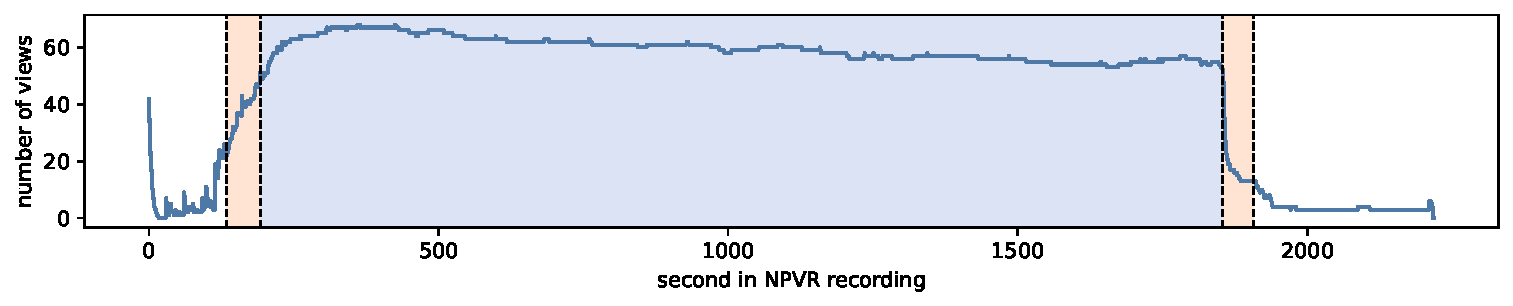
\includegraphics[width=1\textwidth]{../plots/sitcom.pdf}
       \caption{30 min sitcom episode without advertisements, 100 views}
       \label{fig:sitcom_viewing_behaviour} 
    \end{subfigure}
    \par\bigskip
    \begin{subfigure}[b]{\textwidth}
       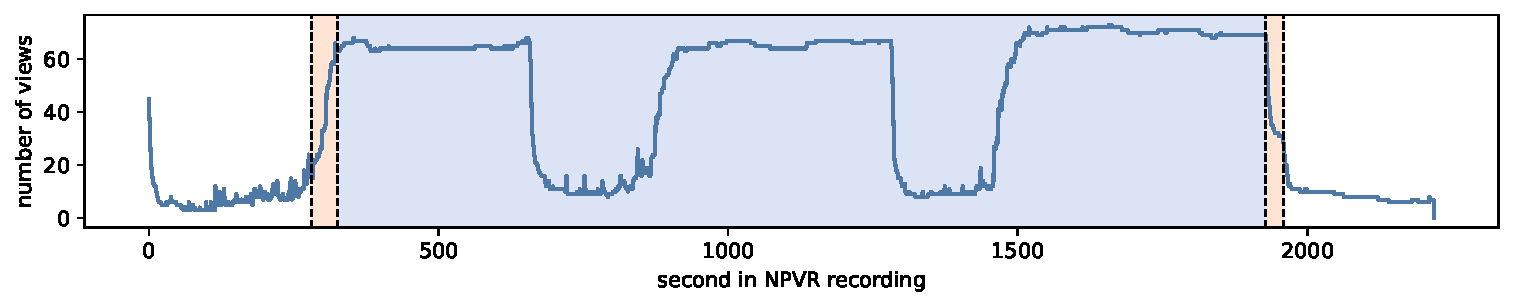
\includegraphics[width=1\textwidth]{../plots/soap_opera.pdf}
       \caption{30 min soap opera episode with two advertisement breaks, 100 views}
       \label{fig:soap_opera_viewing_behaviour}
    \end{subfigure}
    \caption{Visualisation of user viewing behaviour for two example recordings.}
    \label{fig:user_viewing_behaviour}
\end{figure}

% example
Two examples of user viewing behaviour data are illustrated in Figure \ref{fig:user_viewing_behaviour}. The data in both figures consists of a sample of 100 user views, but the views are from two different TV programs. Figure \ref{fig:sitcom_viewing_behaviour} views are from a sitcom episode and Figure \ref{fig:soap_opera_viewing_behaviour} views are from an episode of a soap opera. The episodes are divided into one second-long segments, and calculated for each segment is the number of user views in which the segment was watched. The segments are plotted on the horizontal axis, and the number of user views per segment is plotted on the vertical axis. For example, 63 users from the sample of 100 users watched the part of the sitcom episode between 0:10:00 - 0:10:01 (600 on the horizontal axis in Figure \ref{fig:sitcom_viewing_behaviour}).

The background colour in the figure represents the content type of the time segment: non-program content is white, core program content is blue and beige indicates the opening and closing credits. The change points are marked with a vertical dashed line. There is a distinct increase in the number of views during the opening credits in both figures. Likewise, there is a steep decrease in the number of views during closing credits. The program visualised in Figure \ref{fig:soap_opera_viewing_behaviour} has two advertisement breaks, which appear as recesses in the number of views during the core program content. Figure \ref{fig:sitcom_viewing_behaviour} episode has no advertisement breaks.

\subsection{Data cleaning} \label{subsec:cleaning} % or data cleansing 
% 1. n first views are chosen to simulate real life use case
% 2. view has (player source) duration, filter out views where its value is
%    - not defined
%    - negative
%    - very large
% 3. filter out views which ended before the recording process ended
% 4. filter out views that do not have any skips

% considerations for sample size
% - for a small sample size bad views have a bigger proportional effect to result
% - collecting big sample takes more time and is computationally slightly heavier

% why sample size of 100
This section explains how the sample views were chosen. A uniform sample size was used for all recordings in order to simplify result evaluation and comparison. The characteristic pattern for viewing behaviour, described at the end of the previous section, is usually visible from a dozen views. Sample size of 100 views was chosen because it should be large enough to ensure that it is very unlikely that the characteristic pattern does not emerge.

As the first step, all views of a recording are sorted from oldest to newest. The views will be added to the sample in this order, but potentially incorrect or irrelevant views are filtered out. This means that the sample views are not simply the 100 earliest ones. Firstly, views which end before the recording process ends are discarded. Also views with no skips are discarded, since the change point detection relies on inspecting which parts the viewers skip, so views without skips are useless. Lastly, views with implausible player source duration are removed. This includes the cases where player source duration does not exist, it is negative or close to maximum value for unsigned 32-bit integer.
%TODO: consider filtering out views that are very short

\newpage
\section{Theoretical background} \label{sec:background}

\subsection{Signal change detection} \label{subsec:theory} % for this specific case

%definition
%classification:
%methods (the paper, bayes, something else)
%online/offline
%(un)known nof points 
%cost function, parametric/non-parametric
%search method, optimal/approximate (accuracy vs performance)

% this problem -> signal processing problem -> change point detection problem
% online/offline
% offline -> number of changes known/unknown

%tie to npvr case & definition
Locating the start and end of programs with user viewing behaviour time series data can be formulated as a signal processing problem, more precisely as a change point detection problem. Signal change point detection is quite widely researched topic, since it has applications in multiple fields, such as network traffic data analysis \cite{levy-leducDetectionLocalizationChangepoints2009} \cite{lung-yut-fongDistributedDetectionLocalization2012}, bio-informatics \cite{liuChangepointDetectionMethod2018} \cite{vertFastDetectionMultiple2010} and climatology \cite{reevesReviewComparisonChangepoint2007} \cite{verbesseltDetectingTrendSeasonal2010a}. However, signal processing is not the only possible approach for time series change point detection. Statistical approaches, such as Bayesian methods, are also widely used \cite{barryBayesianAnalysisChange1993} \cite{rabinerTutorialHiddenMarkov1989}, but in order to narrow down the scope of this thesis only signal processing methods will be examined.

The signal in this case is the user viewing behaviour time series data, as described in Section \ref{sec:data}. The assumption in signal change point detection is that the signal consists of segments with different statistical properties, for example a different central tendency. The data in each segment is approximately homogeneous in respect to the statistical property that varies between segments. Change points are the transition points between segments.

% offline
Signal change point detection problems can be divided into two main categories, depending on whether the change detection must be done for incoming data in near real-time, or not. Methods solving the former case are referred to as online algorithms. Offline algorithms solve the latter case, and they differ from the online algorithms by getting the entire dataset as input and typically being computationally more complex, but also by detecting the changes more accurately. The user viewing behaviour data is aggregated from multiple views after the views have ended, meaning that all the data to be analysed is available from the start, allowing offline methods to be used.
%TODO: source for computational complexity
%TODO: keskitytään pelkkiin offline metodeihin

% number of change points
Offline change point detection methods can be divided further into two categories, based on whether the number of change points in the signal, $K$, is known beforehand, or not. If $K$ is unknown, a constraint which restricts the number of change points must be added to prevent overfitting. This is referred to as the \textit{complexity penalty}. There are multiple approaches for choosing the complexity penalty.

% paperi, cost function ja seatch method
Literature review by Truong et al. \cite{truongSelectiveReviewOffline2020} compared a selection of offline change point detection algorithms. It classified the algorithms according to whether the number of change points is known in advance, how the homogeneity within signal segments is measured, and how the signal is divided into segments. The measure of homogeneity is referred to as \textit{cost function} and the method for choosing segments is referred to as \textit{search method}. A more detailed definition of the cost function is in Section \ref{subsec:costfunction} and of the search function in Section \ref{subsec:searchmethod}. The objective of the change point detection algorithms discussed in the literature review is to find a segmentation that minimises the sum of cost functions for the segments. The function to be minimised can be expressed as follows:
\begin{equation}
  \sum_{k=0} ^{K}  \cost(y[t_k+1,t_{k+1}])
  \label{eq:minimise_segments}
\end{equation}
where $y[t_k+1,t_{k+1}]$ is a segment of signal $y$ from index $t_k+1$ to $t_{k+1}$ and $t_{k+n}$ is the index of the $n$th change point, $\cost$ is the cost function, and $K$ is the number of change points.

\subsection{Cost function} \label{subsec:costfunction}

What is a good cost function depends on what kind of change occurs in the signal on change points. Looking at the user viewing behaviour data discussed in Section \ref{sec:data}, it seems that what best describes what happens to the viewer count during credits is a shift in the distribution mean. A cost function that works well for mean shift detection is squared deviation, $\cost_{L_2}$. It measures the variance and is defined as follows:
\begin{equation}
  \cost_{L_2}(y[a,b]) = \sum^b_{t=a} \left\lVert y[t]-\overline{y}[a,b] \right\rVert ^2_2
    \label{eq:l2} \text{,}
\end{equation}
where $y[a,b]$ is a segment of signal $y$ from index $a$ to $b$, and  $\overline{y}[a,b]$ is the empirical mean of $y[a,b]$.

Another possibly suitable cost function for the data is the absolute deviation, $\cost_{L_1}$. It detects changes in the median and can be used also for detecting shifts in other central tendencies, such as mean and mode. It is defined as follows:
\begin{equation}
  \cost_{L_1}(y[a,b]) = \sum^b_{t=a+1} \left\lVert y[t]-\overline{y}[a,b] \right\rVert_1 \text{.}
  \label{eq:l1}
\end{equation}

The key difference between squared deviation and absolute deviation is that the squared deviation penalises larger deviations from the mean more. As there might be some fluctuation in the viewer count during the core program content, and drastic changes in the viewer count typically occur during content type changes, it can be assumed that for this use case Equation \ref{eq:l2} should produce better results than Equation \ref{eq:l1}.

\newpage
\subsection{Search method} \label{subsec:searchmethod}

% optimal vs approximate, why optimal only
Truong et al. \cite{truongSelectiveReviewOffline2020} divided search methods into two categories, by whether they always provide an optimal solution for change point location with the chosen cost function, or if they provide an approximate solution. This thesis will examine only optimal methods. Optimal methods produce inherently more reliable and accurate results than approximate ones, with the trade-off of typically higher computational complexity. The approximate methods are excluded on the basis that the goal of this thesis is to study whether it is at all possible to detect credits from solely viewing behaviour statistics, not determining the most viable approach to do it in practice. Therefore, high reliability and accuracy outweighs low computational complexity.

% (un)known k
Two optimal search methods were presented in the literature review, \texttt{Opt} and \texttt{Pelt}. \texttt{Opt} was first introduced by Bellman \cite{bellmanRoutingProblem1958} for an unrelated problem. \texttt{Pelt}, short for Pruned Exact Linear Time, was first introduced by Killick et al. \cite{killickOptimalDetectionChangepoints2012}. The main difference between the methods is that \texttt{Opt} requires the number of change points $K$ to be known beforehand, and \texttt{Pelt} can be used when $K$ is unknown.

%dynamic programming
Both of the methods use dynamic programming to find the change points. Dynamic programming is a mathematical optimisation method, where the problem is solved by recursively dividing it into smaller sub-problems. In this case the problem is minimising Equation \ref{eq:minimise_segments}. The optimal segmentation is defined as follows:
\begin{equation}
  \OPT([a,b],K): \text{Optimal segmentation for } y[a,b] \text{ with $K$ change points} 
\label{eq:opt}
\end{equation}
When $K$ is known in advance the optimal segmentation can be calculated as follows:

The recursive step:
\begin{equation}
  \OPT([a,b],K) = \min\limits_{a<k<b}
    \begin{cases}
      \cost(y[a,k]) \hspace{0.1cm}+ \\
      \OPT([k+1,b],K-1)
    \end{cases}
\label{eq:recursivestep}
\end{equation}
The base case:
%base case
\begin{equation}
  \text{For all 1} \leq a < b \leq m:
    \OPT([a,b],0) \leftarrow \cost(y[a,b]) \text{,}
\label{eq:basecase}
\end{equation}
where $m$ is the number of elements in $y$.

Intuitively, the above equations can be understood as follows. The base case in Equation \ref{eq:basecase} occurs when there are no change points and thus no subsegments, that is $K=0$. For a signal with no change points, Equation \ref{eq:minimise_segments} is simply the output of the cost function for that signal. Finding the optimal segmentation for a signal with $K > 0$ change points means finding a set of segments that minimises the sum of costs. As described in Equation \ref{eq:recursivestep}, the minimisation task can be expressed as finding the optimal combination of the first segment and optimal segmentation for the remaining signal.

The concept of the algorithm is represented as top-down, but in practice the implementa-tion is done bottom-up, by first computing the possible base cases and building more complex optimal segmentations on top of the simpler ones with less change points.

% pelt
In principle, finding the optimal set of change points works similarly when $K$ is unknown. It would be possible to choose a sufficiently large maximum value $K=K_{\text{max}}$ and iterate \texttt{Opt} for all $K=1\text{, ..., }K_{\text{max}}$ and choose the result which produced the best minimisation of Equation \ref{eq:minimise_segments}. However, the computational complexity of this method is very high. A more viable solution is to add a complexity penalty term into Equation \ref{eq:minimise_segments} to restrict the number of predicted change points. With the complexity penalty $\pen$ Equation \ref{eq:minimise_segments} becomes:
\begin{equation}
  \sum_{k=0} ^{K} \left[ \cost(y[t_k+1,t_{k+1}]) + \pen \right]
  \label{eq:minimise_segments_pen}
\end{equation}
When $\pen$ is linear the \texttt{Pelt} algorithm can be used. In principle, \texttt{Pelt} follows the dynamic programming approach of Equation \ref{eq:recursivestep} and \ref{eq:basecase}, but there is a pruning rule which discards some indices which cannot be change points, reducing the computational complexity. \cite{killickOptimalDetectionChangepoints2012}
%TODO: exact computational complexity
%TODO: explain pruning rule in more detail
%TODO: explain different penalties

\newpage
\section{Methods} \label{sec:casestudy}

\subsection{Sample data and ground truth} \label{subsec:groundtruth}

In order to evaluate how well a method detects change points, a ground truth is needed for comparison. Ground truth can be obtained by having a person look at a video recording and having them write down the timestamps of the change points.

The start and end time of both opening and closing credits were collected by hand from 279 NPVR recordings with a margin of error of $\pm$ 1 seconds. The sample consists of episodes from 16 different TV series. 138 of the sample recordings were broadcast on non-commercial channels, and therefore they do not contain advertisement breaks. Some general information about these recordings is listed in Table \ref{tab:data_no_ads}. The 141 recordings with advertisement breaks are listed in Table \ref{tab:data_ads}. Every recording in the sample has at least one hundred user views, after the data cleaning process described in Section \ref{subsec:cleaning}. 

The reason for selecting exclusively serial programs in the sample is that series tend to have a predictable program structure that stays consistent between episodes. This makes it faster to collect the ground truth, as the program structure has to be deciphered only once per series. For the rest of the episodes, the person collecting the timestamps knows what to look for.

There were a couple of factors that contributed to a series being included in the sample. These were the perceived likelihood of the series being popular enough to have a least one hundred suitable user views per episode, a large amount of episodes, and a conventional program structure in which credits are clearly distinct from the program content. Nevertheless, some series were included in the sample mostly by chance.

The sample series were categorised by program structure. The categories are defined in Table \ref{tab:structure}. Conventional program structure refers to both of the credits being clearly distinct from the core program content, and in between the non-program and core program content. For example, the program in Figure \ref{fig:sitcom_viewing_behaviour} has conventional structure. The other categories refer to some anomaly in the program structure, compared to the conventional structure.

Recapitulations of previous episodes and sneak peeks into following episodes were considered as a part of the credits in the ground truth. For programs with a delayed or entwined intro, the ground truth for opening credits was set to consist of the first second of the program, instead of the actual opening credits. The reasoning behind this was the assumption, that an average viewer does not want to miss the first minutes of the core program content before or during the opening credits. For programs with split intro, the ground truth opening credits contains only the first part of the opening credits.

\begin{table}[H]
  \begin{center}
    \begin{tabular}{|c|c|c|c|c|}
      \hline
      \textbf{series} & \textbf{episodes} & \textbf{episode length} & \textbf{genre} & \textbf{structure}
      \\ \hline
      A &  6 & 30 min & reality television & conventional
      \\ \hline
      B & 10 & 30 min & comedy & conventional
      \\ \hline
      C & 32 & 30 min & comedy & conventional
      \\ \hline
      D & 30 & 45 min & drama & conventional
      \\ \hline
      E &  8 & 50 min & drama & conventional
      \\ \hline
      F & 20 & 50 min & drama & conventional
      \\ \hline
      G &  4 & 45 min & drama & \hspace{3.3mm}conventional *
      \\ \hline
      H & 3 & 90 min & drama & entwined intro
      \\ \hline
      I &  9 & 40 min & drama & recap, split intro
      \\ \hline
      J &  16 & 45 min & drama & split intro
      \\ \hline
    \end{tabular}
  \end{center}
  \caption{Sample recordings without advertisement breaks categorized by series.}
  \label{tab:data_no_ads}
\end{table}

\begin{table}[H]
  \begin{center}
    \begin{tabular}{|c|c|c|c|c|c|}
      \hline
      \textbf{series} & \textbf{episodes} & \textbf{ad breaks} & \textbf{episode length} & \textbf{genre} & \textbf{structure}
      \\ \hline
      K & 35 & 1 & 30 min & soap opera & conventional
      \\ \hline
      L & 25 & 1 & 30 min & soap opera & delayed intro
      \\ \hline
      M & 15 & 1, 2 or 3 & 30-60 min & reality television & recap, sneak peek
      \\ \hline
      N &  9 & 4 & 90 min & reality television & recap, sneak peek
      \\ \hline
      O & 31 & 2 & 30 min & soap opera & sneak peek
      \\ \hline
      P & 26 & 3 & 50 min & drama & split intro
      \\ \hline
    \end{tabular}
  \end{center}
  \caption{Sample recordings with advertisement breaks categorized by series.}
  \label{tab:data_ads}
\end{table}

\begin{table}[H]
  \begin{center}
    \begin{tabular}{|c|p{12.3cm}|}
      \hline
      \textbf{category} &  \hspace{0.5cm} \textbf{description}
      \\ \hline
      conventional & Distinct opening and closing credits.
      \\ \hline
      delayed intro & Opening credits occur a few minutes after the program has begun. 
      \\ \hline
      entwined intro & Opening credits are entwined with the core program content.
      \\ \hline
      recap & Program begins with a recapitulation of the previous episode.
      \\ \hline
      sneak peek & Closing credits end with a sneak peek into the following episode.
      \\ \hline
      split intro & Opening credits are divided in two parts. The first part is at the beginning of the program, and the second occurs a few minutes after the program has begun.
      \\ \hline
    \end{tabular}
  \end{center}
  \caption{Descriptions of the program structure categories.}
  \label{tab:structure}
\end{table}

\begin{center}
* One episode has delayed intro, rest of the episodes have conventional structure.
\end{center}

\subsection{Change point detection with the \texttt{ruptures} library} \label{subsec:solution}

% what is ruptures
Change points were detected from the sample data with the Python library \texttt{ruptures}. The library is based on the findings of the Truong et al. literature review \cite{truongSelectiveReviewOffline2020}. Selected algorithms examined in the literature review are implemented in \texttt{ruptures}.

% search method should be optimal 
Suitable algorithms for this use case were chosen by considering the three aspects of change point detection methods discussed in the literature review: cost function, search method and complexity penalty. In this case accuracy is more important than low computational complexity, so optimal method is preferable to an approximate one. Two optimal search methods, \texttt{Opt} and \texttt{Pelt}, are implemented in \texttt{ruptures}, as described in Section \ref{subsec:searchmethod}.

% opt vs pelt
As mentioned in Section \ref{sec:data}, advertisement breaks in the recording may produce recesses in the viewer count. Change point detection algorithms can interpret these recesses as separate segments. The number of advertisement breaks per program varies, meaning that $K$ is unknown if the recording might contain advertisement breaks. However, programs in non-commercial channels never contain advertisements, and for them, it was assumed that there should be exactly one change point at the beginning and one at the end of the program. This implies that \texttt{Opt} should be a viable search method for recordings from non-commercial channels with $K=2$. \texttt{Pelt} can be used for all the recordings, but the complexity penalty needs to be calibrated. The penalty was calibrated heuristically, and the calibration process that was used is described in Section \ref{sec:results_pelt}.

% cost function
The \texttt{ruptures} library has three different cost functions that can be used with \texttt{Opt} and \texttt{Pelt}. These are absolute deviation $\cost_{L1}$ as described in Equation \ref{eq:l1}, squared deviation $\cost_{L2}$ as described in Equation \ref{eq:l2}, and kernel cost function $\cost_{\text{rbf}}$. $\cost_{\text{rbf}}$ was not taken into further consideration, because it is substantially more complex than the other two cost functions. 
$\cost_{L2}$ is preferable over $\cost_{L1}$, for the reasons discussed in section \ref{subsec:costfunction}. 

Standard statistical methods for univariate analysis were used for result evaluation. The statistics include five-number summary first devised by Tukey et al. \cite{tukeyExploratoryDataAnalysis1977a}, which includes the median, the 1st and 3rd quartiles and the minimum and maximum.

\newpage
% notation
Following the convention used by Truong et al. the actual change points are denoted by $t$ and the change points produced by \texttt{ruptures} are denoted by $\hat{t}$ \cite{truongSelectiveReviewOffline2020}. Each change point has a subscript, where the first letter denotes the credits the change point corresponds to ($o$: opening credits, $c$: closing credits). If there are separate change points for the start and end timestamps of the credits, the subscript will have a second letter that denotes which one of those the change point represents ($s$: start, $e$: end). This notation is illustrated in Figure \ref{fig:change_point_notation}.

\begin{figure}[H]
    \centering
    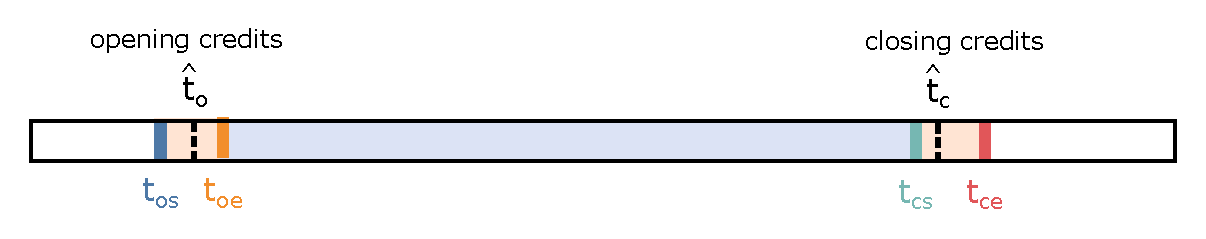
\includegraphics[width=1\textwidth]{../plots/timeline.pdf}
    \caption{Notation for the actual ( $t$ ) and predicted ( $\hat{t}$ ) change points.}
    \label{fig:change_point_notation}
\end{figure}

\newpage
\section{Results} \label{sec:results}

\subsection{Non-commercial channels with \texttt{Opt} as search method} \label{sec:results_opt}

% output visualisation & comparison to ground truth fig
% yleiskuva siitä millaista settiä rupturesta tulee ulos
An example of \texttt{Opt} output with cost function $\cost_{L2}$ and number of change points $K=2$ is visualised in Figure \ref{fig:opt_sitcom}. The viewing behaviour data is the same as in Figure \ref{fig:sitcom_viewing_behaviour}. The difference between the figures is that in Figure \ref{fig:opt_sitcom} the vertical dashed lines mark the change points determined by \texttt{ruptures} instead of the actual change points checked by hand. In the example, both of the predicted change points align with the credits. The change point for the start of the program is in the middle of the opening credits and the change point for the end of the program is close to the beginning of the closing credits.

\begin{figure}[h]
  \centering
  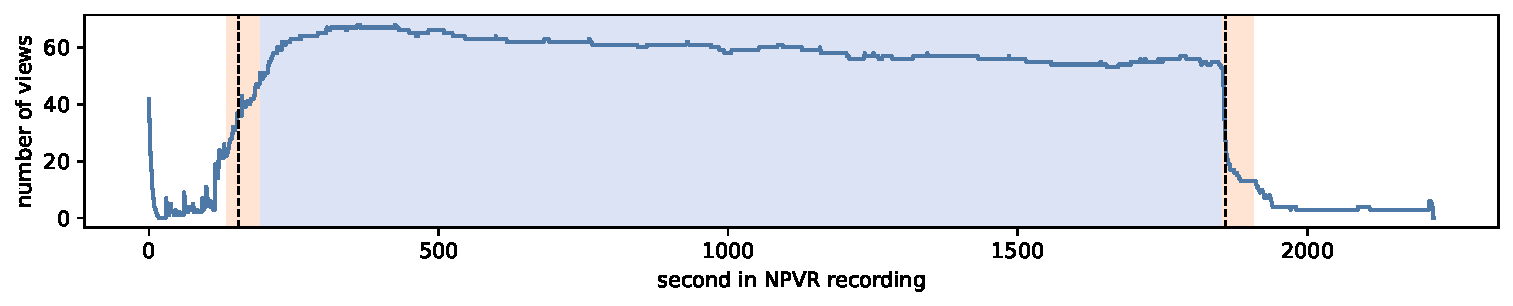
\includegraphics[width=1\textwidth]{../plots/sitcom-pelt_l2_pen30000.pdf}
  \caption{\texttt{Opt} $\cost_{L2}$ $K=2$ output for Figure \ref{fig:sitcom_viewing_behaviour} data.}
  \label{fig:opt_sitcom}
\end{figure}

Running \texttt{Opt} $\cost_{L2}$ with $K=2$ for Table \ref{tab:data_no_ads} recordings, it turns out that in most cases the results are quite similar to Figure \ref{fig:opt_sitcom}, and the predicted change points typically land somewhere on the credits. Out of the 138 recordings, the first change point landed outside of opening credits in 25 recordings
and the second change point was not on the closing credits in one recording. More statistics of the result are listed in Table \ref{tab:statistics_opt}.

\begin{table}[h]
  \begin{center}
  \begin{tabular}{|c|c|c|c|c|}
      \hline
      \textbf{statistic} & $\hat{t}_o-t_{os}$ & $\hat{t}_o-t_{oe}$ & $\hat{t}_c-t_{cs}$ & $\hat{t}_o-t_{os}$  \\ \hline
      minimum & -22 & -65 & 3 & -107\\ \hline
      1st quartile & 9 & -17.75 & 5 & -50.75\\ \hline
      median & 16 & -7 & 7 & -35.5\\ \hline
      3rd quartile & 45,75 & -5 & 8 & -28 \\ \hline
      maximum & 157 & 152	& 36 & 5\\ \hline
      variance & 676 & 635	& 17.2 & 873\\ \hline
      standard deviation & 26.0 & 25.2 & 4.15 & 29.5\\ \hline
  \end{tabular}
  \end{center}
  \caption{Five-number summary and other statistics for \texttt{Opt} $\cost_{L2}$ $K=2$.}
  \label{tab:statistics_opt}
\end{table}
% TODO: add outside of credits row

The assumption stated in Section \ref{subsec:solution}, that the lack of advertisement breaks would result in $K=2$ change points being aligned to the start and end of the program, did not hold for all the recordings. For two episodes of series J and one episode of series H, from Table \ref{tab:data_no_ads}, the first change point is off by a couple of minutes. In series J the change point is on the delayed opening credits and in series H during the opening credits entwined with the core program content. This explains the large maximum value for $\hat{t}_o-t_{oe}$ in Table \ref{tab:statistics_opt}. Without these three outliers the maximum value for $\hat{t}_o-t_{oe}$ would be 11.

The five-number summary of the quartiles in Table \ref{tab:statistics_opt} gives some insight about the output, but the results can be understood more intuitively by plotting the data. Plotted in Figure \ref{fig:t_diff_opt_credits} are the predicted locations for opening and closing credits, $\hat{t}_o$ and $\hat{t}_c$, compared to the actual start and end times of the credits. Figure \ref{fig:t_diff_opt_os} has $\hat{t}_o-t_{os}$ values plotted, Figure \ref{fig:t_diff_opt_oe} has $\hat{t}_o-t_{oc}$ values plotted, et cetera.

\begin{figure}[h]
  \begin{subfigure}[t]{.49\textwidth}
    \centering
    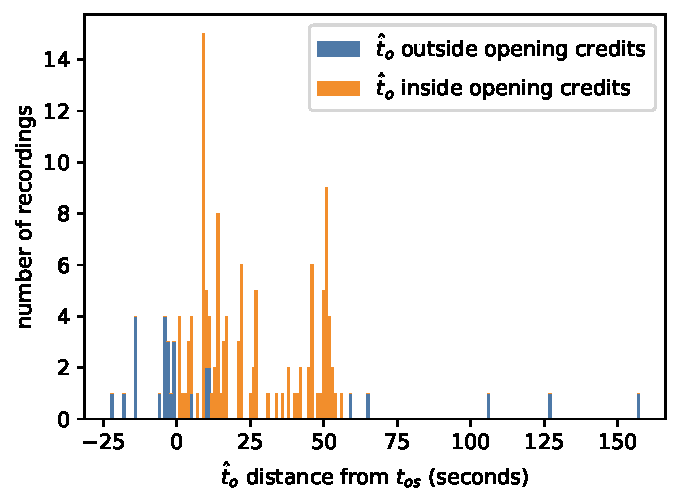
\includegraphics[width=\linewidth]{../plots/distances/opt_l2_dist_start_first.pdf}
    \caption{Start of opening credits}
    \label{fig:t_diff_opt_os}
  \end{subfigure}
  \hfill
  \begin{subfigure}[t]{.49\textwidth}
    \centering
    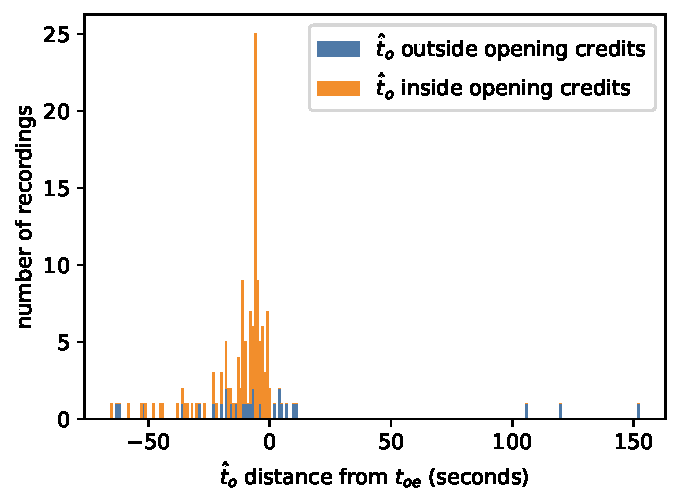
\includegraphics[width=\linewidth]{../plots/distances/opt_l2_dist_start_last.pdf}
    \caption{End of opening credits}
    \label{fig:t_diff_opt_oe}
  \end{subfigure}
  \begin{subfigure}[t]{.49\textwidth}
      \centering
      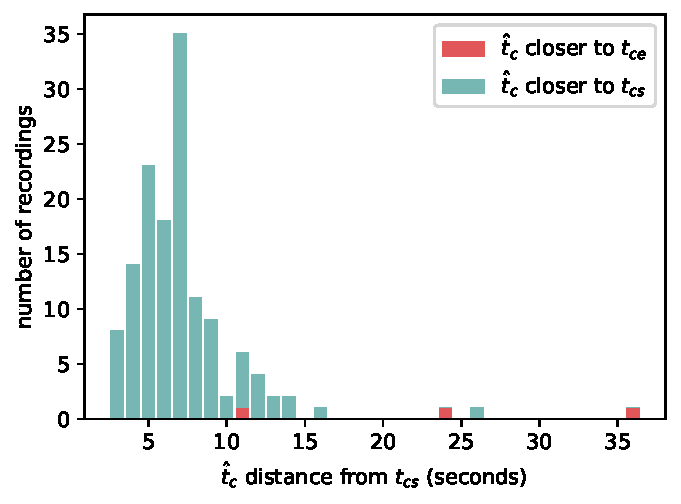
\includegraphics[width=\linewidth]{../plots/distances/opt_l2_dist_end_first.pdf}
      \caption{Start of closing credits}
      \label{fig:t_diff_opt_cs}
    \end{subfigure}
    \begin{subfigure}[t]{.49\textwidth}
      \centering
      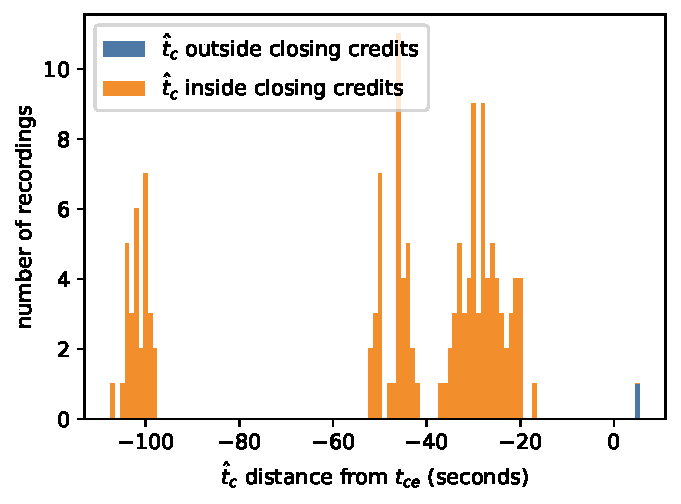
\includegraphics[width=\linewidth]{../plots/distances/opt_l2_dist_end_last.pdf}
      \caption{End of closing credits}
      \label{fig:t_diff_opt_ce}
    \end{subfigure}
  \caption{\texttt{Opt} $\cost_{L2}$ $K=2$ output compared to actual change points of credits.}
  \label{fig:t_diff_opt_credits}
\end{figure}

In order to gain more insight about the results, the change points were divided into two categories, depending on whether the predicted change point $\hat{t}$ is within the credits it corresponds to, or not. Both $\hat{t_o}$ and $\hat{t_c}$ are typically somewhere on the credits, but $\hat{t_o}$ has more predictions outside the credits and higher variance in the relative position within the credits. For the closing credits, it is visible in Figure \ref{fig:t_diff_opt_cs} and \ref{fig:t_diff_opt_ce} that most often $\hat{t}_c$ is very close to $t_{cs}$, although with a delay of a few seconds. Three fourths of the sample $\hat{t}_c$ results are within $8$ $s$ from $t_{cs}$. Another detail worth noting is that 
it holds for all samples that $ \hat{t}_c > t_{cs}$, meaning that none of the $\hat{t}_c$ were predicted to be before the closing credits.

The relative position of the predicted change points within the credits is visualised in Figure \ref{fig:relative_opt}. The position $0.0$ on the x-axis marks the beginning of credits and position $1.0$ marks the end of credits. From Figure \ref{fig:relative_opening_opt} it can be seen that $\hat{t}_o$ is more often closer to $\hat{t}_{oe}$ than $\hat{t}_{os}$, but it aligns strongly with neither. However, $\hat{t}_c$ has a clear tendency to align with $\hat{t}_{cs}$ with a slight time delay, as seen in Figure \ref{fig:relative_closing_opt}. Credits that are ten seconds long or shorter were left out of the visualisation, because for very short credits misprediction by a few seconds is a big error compared to the length of the credits, which easily disturbs the clarity of the visualisation.

\begin{figure}[h]
  \begin{subfigure}[t]{.49\textwidth}
    \centering
    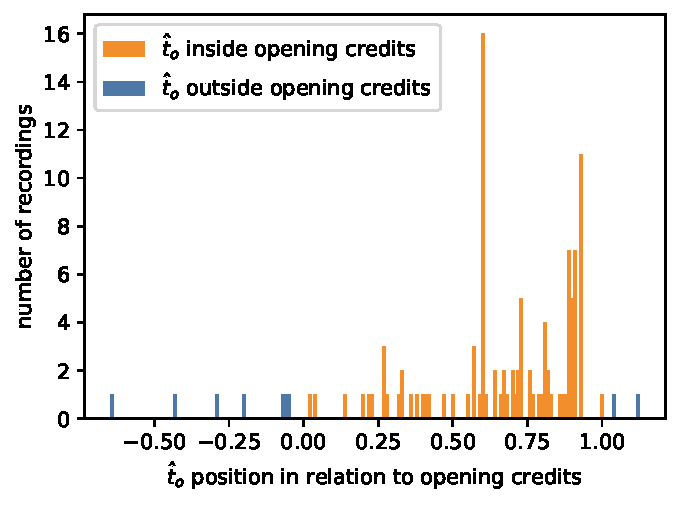
\includegraphics[width=\linewidth]{../plots/distances/relative_opening_opt.pdf}
    \caption{Opening credits}
    \label{fig:relative_opening_opt}
  \end{subfigure}
  \hfill
  \begin{subfigure}[t]{.49\textwidth}
    \centering
    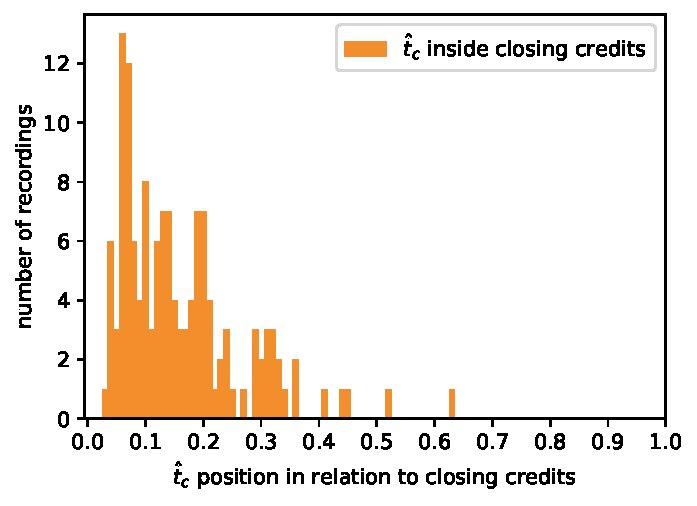
\includegraphics[width=\linewidth]{../plots/distances/relative_closing_opt.pdf}
    \caption{Closing credits}
    \label{fig:relative_closing_opt}
  \end{subfigure}
  \caption{\texttt{Opt} $\cost_{L2}$ $K=2$  output change point position in relation to credits.}
  \label{fig:relative_opt}
\end{figure}

\subsection{All channels with \texttt{Pelt} as search method} \label{sec:results_pelt}

As the number of change points detected by \texttt{Pelt} is controlled by a complexity penalty, the exact amount of detected change points is not known in advance. A common outcome is that one change point is predicted per credits, possibly with additional change points within the program. Occasionally the output is more precise, and both the start and end of credits are found. An example of this is visualised in Figure \ref{fig:intro_good}. However, as can be seen in Figure \ref{fig:intro_bad}, sometimes results that seem possibly very accurate can be misleading. Since there is no trivial way to evaluate whether \texttt{Pelt} output is more accurate than usually, without knowing the ground truth, only the first and last predicted change points of recordings were examined, and it was assumed that the former corresponded to opening credits, and the latter to closing credits.

\begin{figure}[h]
  \centering
  \begin{subfigure}[b]{\textwidth}
     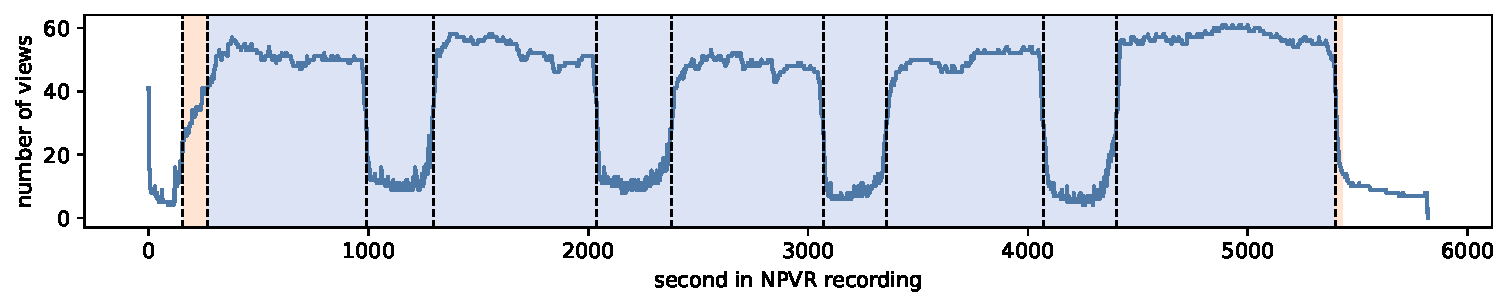
\includegraphics[width=1\textwidth]{../plots/intro_good.pdf}
     \caption{Start and end of opening credits are identified correctly}
     \label{fig:intro_good} 
  \end{subfigure}
  \par\bigskip
  \begin{subfigure}[b]{\textwidth}
     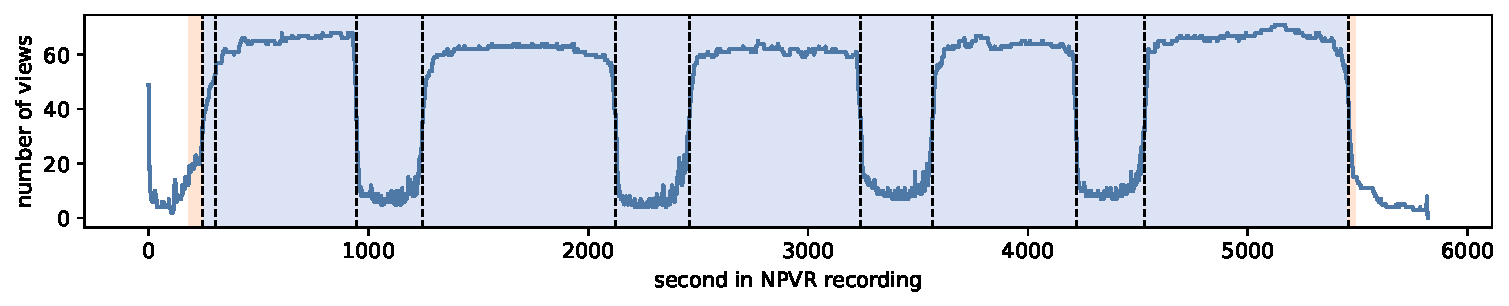
\includegraphics[width=1\textwidth]{../plots/intro_bad.pdf}
     \caption{End of opening credits is correctly identified, but with an extra change point after it}
     \label{fig:intro_bad}
  \end{subfigure}
  \caption{\texttt{Pelt} $\cost_{L2}$, $\pen=18000$, output for two episodes of series N from Table \ref{tab:data_ads}.}
  \label{fig:intro_pelt}
\end{figure}

The value for the $\cost_{L_2}$ complexity penalty was determined heuristically, by trying out different values and evaluating the result with the following criterion: a complexity penalty was considered sufficiently good, when for all the 279 sample recordings, both the first and last predicted change point were within 60 seconds of the opening or closing credits, respectively. Penalties between 10000 and 25000 produced good results, when the penalty was increased in increments of one hundred. It can be assumed that, for the sample data, penalties smaller than 10000 are prone to detect too many change points, and likewise penalties larger than 25000 are likely to fail to detect all relevant changes. Penalty of 18000 was chosen as the final value, because it is almost in the middle of 10000 and 25000, and thus it is likely to minimise the risk for both under and oversegmentation.

Statistics of the results with \texttt{Pelt} $\cost_{L_2}$, pen=180000 are listed in Table \ref{tab:statistics_pelt}. The data encompasses all the 279 recordings in Table \ref{tab:data_no_ads} and \ref{tab:data_ads}. The absolute distance from the beginning and end of credits is plotted in Figure \ref{fig:t_diff_credits} similarly as the \texttt{Opt} results in Figure \ref{fig:t_diff_opt_credits}. The relative distance within credits is plotted in Figure \ref{fig:relative}. Similar to Figure \ref{fig:relative_opt}, in order to keep the visualisation informative, credits that are ten seconds long or shorter were excluded from Figure \ref{fig:relative}.

The results appear to be quite similar to the results with \texttt{Opt}. This is not surprising, as both \texttt{Opt} and \texttt{Pelt} are optimal search methods. The optimal nature of the methods implies that, with the same cost function, the output produced by the methods is identical, if the number of change points predicted by \texttt{Pelt} happens to be the same that was given as the parameter $K$ to \texttt{Opt}. For example, if \texttt{Pelt} $\cost_{L_2}$ happened to predict $K=2$ change points for all Table \ref{tab:data_no_ads} recordings, the results would be identical to what is presented in Section \ref{sec:results_opt}. However, as only the first and last change points predicted by \texttt{Pelt} are considered, and the complexity penalty was calibrated with this in mind, \texttt{Pelt} sometimes predicted more change points than \texttt{Opt} for the same recordings. The criterion for choosing the penalty value ensured that the start time of the three recordings that were mispredicted with \texttt{Opt}, was predicted approximately correctly.

\begin{table}[h]
    \begin{center}
    \begin{tabular}{|c|c|c|c|c|}
        \hline
        \textbf{statistic} & $\hat{t}_o-t_{os}$ & $\hat{t}_o-t_{oe}$ & $\hat{t}_c-t_{cs}$ & $\hat{t}_o-t_{os}$ \\ \hline
        minimum & -39 & -161 & 2 & -107 \\ \hline
        1st quartile & 2 & -18.5 & 5 & -44 \\ \hline
        median & 12 & -10 & 7 & -29 \\ \hline
        3rd quartile & 23 & -5 & 9 & -23.5 \\ \hline
        maximum & 100 & 11	& 66 & 9 \\ \hline
        variance & 382 & 471 & 169 & 776 \\ \hline
        standard deviation & 19.6 & 21.7 & 13.0 & 27.9 \\ \hline
    \end{tabular}
    \end{center}
    \caption{Five-number summary and other statistics for \texttt{Pelt} $\cost_{L2}$, $\pen=18000$.}
    \label{tab:statistics_pelt}
\end{table}

\begin{figure}[h]
    \begin{subfigure}[t]{.49\textwidth}
      \centering
      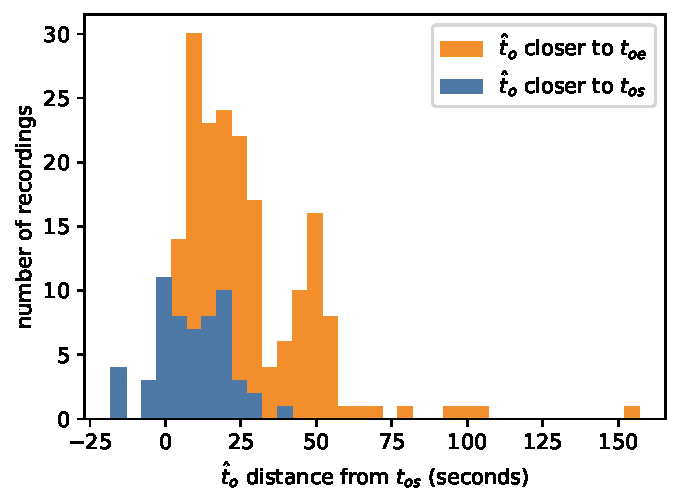
\includegraphics[width=\linewidth]{../plots/distances/pelt_l2_dist_start_first.pdf}
      \caption{Start of opening credits}
      \label{fig:t_diff_os}
    \end{subfigure}
    \hfill
    \begin{subfigure}[t]{.49\textwidth}
      \centering
      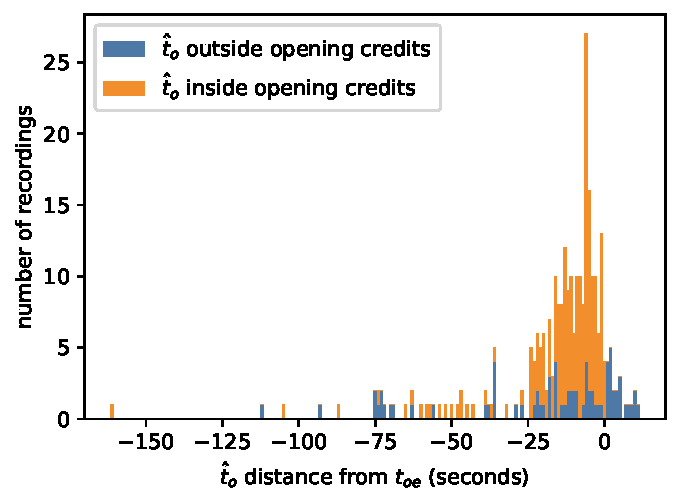
\includegraphics[width=\linewidth]{../plots/distances/pelt_l2_dist_start_last.pdf}
      \caption{End of opening credits}
      \label{fig:t_diff_oe}
    \end{subfigure}
    \begin{subfigure}[t]{.49\textwidth}
        \centering
        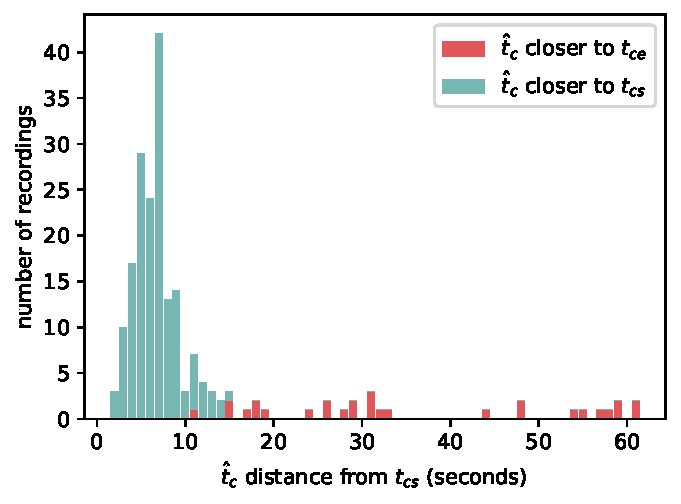
\includegraphics[width=\linewidth]{../plots/distances/pelt_l2_dist_end_first.pdf}
        \caption{Start of closing credits}
        \label{fig:t_diff_cs}
      \end{subfigure}
      \begin{subfigure}[t]{.49\textwidth}
        \centering
        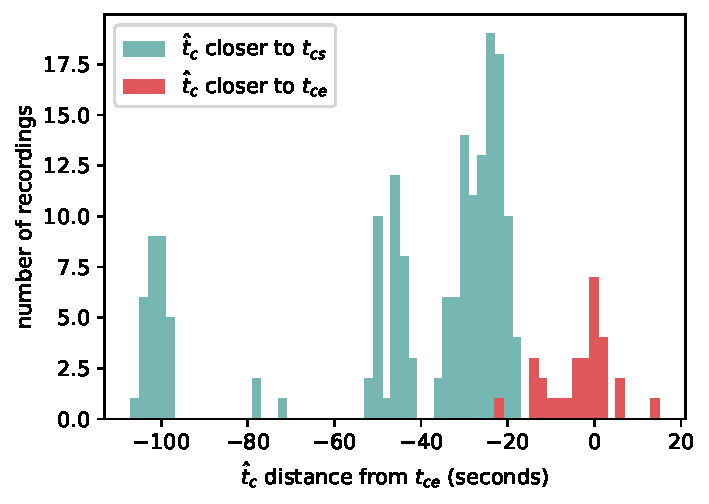
\includegraphics[width=\linewidth]{../plots/distances/pelt_l2_dist_end_last.pdf}
        \caption{End of closing credits}
        \label{fig:t_diff_ce}
      \end{subfigure}
    \caption{\texttt{Pelt} $\cost_{L2}$ $\pen=18000$ output compared to actual change points of credits.}
    \label{fig:t_diff_credits}
\end{figure}

\begin{figure}[h]
  \begin{subfigure}[t]{.49\textwidth}
    \centering
    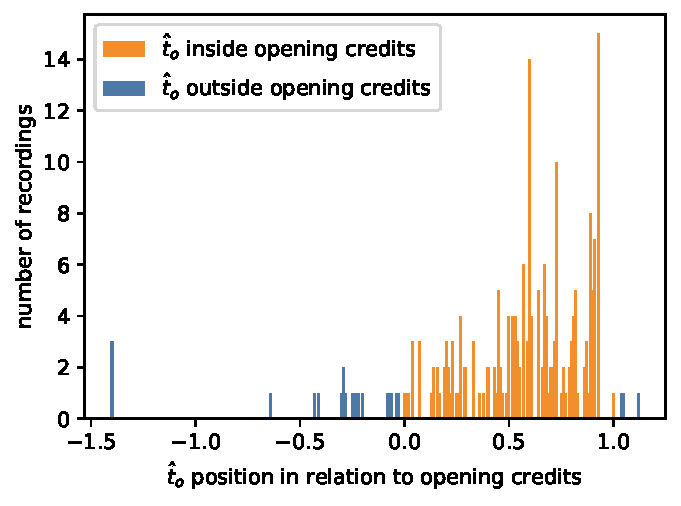
\includegraphics[width=\linewidth]{../plots/distances/relative_opening_pelt.pdf}
    \caption{Opening credits}
    \label{fig:relative_opening}
  \end{subfigure}
  \hfill
  \begin{subfigure}[t]{.49\textwidth}
    \centering
    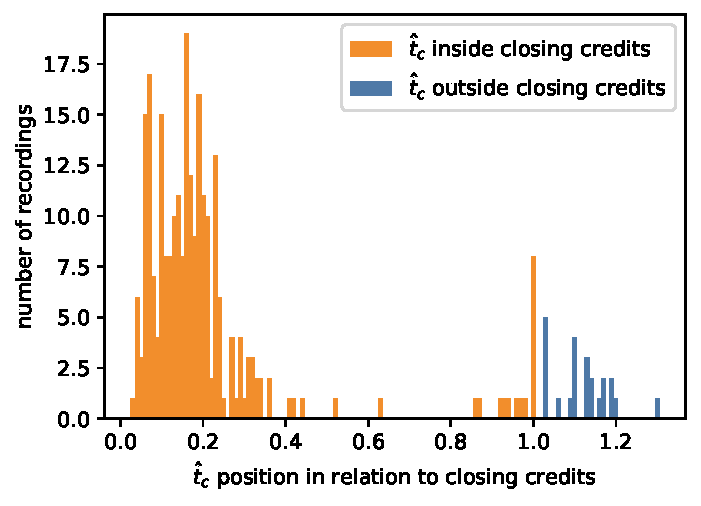
\includegraphics[width=\linewidth]{../plots/distances/relative_closing_pelt.pdf}
    \caption{Closing credits}
    \label{fig:relative_closing}
  \end{subfigure}
  \caption{\texttt{Pelt} $\cost_{L2}$ $\pen=18000$ output change point position in relation to credits.}
  \label{fig:relative}
\end{figure}

One distinct difference between \texttt{Opt} and \texttt{Pelt} output can be seen in the position of $\hat{t}_c$ in relation to closing credits, visualised in Figure \ref{fig:relative_closing_opt} and \ref{fig:relative_closing}. For \texttt{Pelt}, some $\hat{t}_c$ are clustered around the end of the closing credits, which did not happen for \texttt{Opt}. As it happens, this has more to do with the program structure than search method. Plotted in Figure \ref{fig:relative_sneakpeek} is the same data as in Figure \ref{fig:relative_closing}, but the results for the programs with a sneak peek at the end of the closing credits are coloured in red. It can be seen that the cluster around the end of closing credits consists almost solely from these programs. In the sample data all the series with a sneak peek have advertisement breaks, and therefore they were not included in the \texttt{Opt} sample.

\begin{figure}[h]
  \centering
  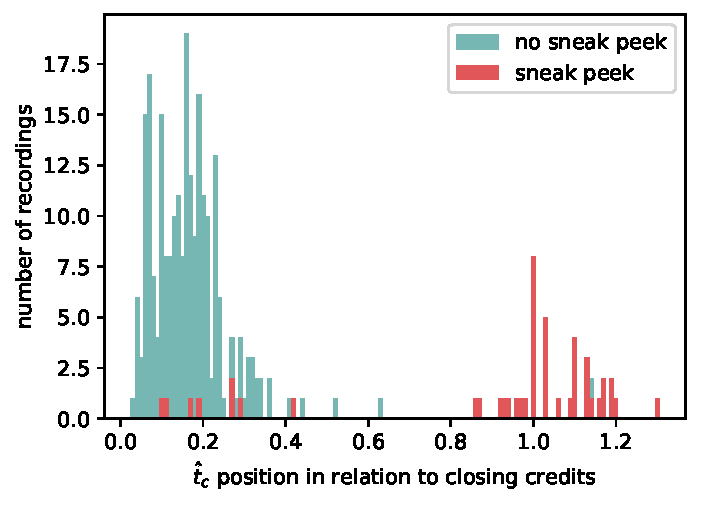
\includegraphics[width=.8\textwidth]{../plots/distances/relative_closing_sneak_peek.pdf}
  \caption{Figure \ref{fig:relative_closing} data with episodes with a sneak peek highlighted}
  \label{fig:relative_sneakpeek}
\end{figure}

\newpage
\section{Discussion} \label{sec:discussion}

\subsection{Interpretation of the results}

The results described in Section \ref{sec:results} show that identifying the approximate location of both opening and closing credits is possible merely with viewing behaviour data. However, the results are not always accurate, and usually only the general location of credits was found, instead of the exact start and end time of the credits.

The assumption was proved false that only advertisement breaks would produce notable recesses in the views count within the program content. 
In Section \ref{sec:results_opt} it was shown that with \texttt{Opt} as the search method unconventional structure of opening credits might cause the start of program to be detected less accurately. Although the first change point was not within one minute of the start of the program only in three recordings out of the 138 recordings in Table \ref{tab:data_no_ads}, it must be concluded that specifying the number of change points to be detected in advance might lead to impaired accuracy. This is true at least if no heuristics are used to evaluate the accuracy of \texttt{ruptures} output.

Results with the \texttt{Pelt} search method were more accurate, but as the complexity penalty was adjusted with the dataset itself, it is possible that the penalty value is overfitted for the data and does not produce generally as good results. However, the range of complexity penalties that got the start and end change points for the program approximately correct was quite wide, and the final penalty value was chosen from the middle of this range. This makes it more likely that the chosen penalty value works also for other recordings.

Unconventional program structure might affect the results, as was seen both with the opening credits in \texttt{Opt} and the closing credits in \texttt{Pelt}. Content that is generally considered interesting is viewed frequently, which is reflected in the location of change points.

\subsection{Possible future considerations}

There are multiple aspects of the credits detection process that could be improved or investigated further. These aspects can be roughly categorised into studying the viability of the concept, improving the computational speed of the process, or improving the accuracy of the results.

Questions regarding the sample size and data cleaning affect both the computational speed and accuracy. It could be investigated what is a sufficient sample size of user views per recording for the characteristic user behaviour pattern to emerge. The data cleaning procedure could possibly be improved by either doing more filtering, in order to get the data to display the characteristic user behaviour pattern more clearly, 
or by filtering less in order to gather the needed amount of views faster. The filtering criteria could be reconsidered, and the data could perhaps be preprocessed  somehow in order to improve the results.

Approximate search methods could be tried out, in order to study whether they produce significantly worse result than \texttt{Pelt}, or if the results are almost as good. Other cost functions than $\cost_{L2}$ could be experimented with, and 
choosing a suitable value for the complexity penalty is a rather vast topic.

Perhaps the biggest question about the viability of the concept is, does the sample data represent all recordings. The sample consisted only of 30-90 min long episodes of TV series, which is a rather narrow subset of all broadcast programs. Short programs, programs that do not belong to a series, and programs from different genres, such as news, sports or documentaries could be tried out. Another variable to consider could be the program structure, although this sample already had programs with opening credits that are not located at the very beginning of the program, recapitulations of previous episodes, and sneak peeks into future episodes at the end of closing credits.

Offline signal change point detection is not the only possible approach for detecting the drastic changes in the viewer count. For example Bayesian methods could also be used, as mentioned in the beginning of Section \ref{subsec:theory}.
The approach examined in this thesis could perhaps be combined with some other approach, or with heuristics about the expected program structure, in order to get more reliable and accurate results.

\subsection{Possible applications}

There are a couple of areas where change points detected from user behaviour data could be useful. Firstly, change point detection could be combined with other methods for identifying video content, in order to find the exact position of credits. For instance, text in credits could be detected with optical character recognition (OCR) \cite{ngoVideoTextDetection2005}. Change point detection from user behaviour could be used to ensure that the text found by OCR belongs to the credits of the entirely recorded program, and not to the closing credits of the previous one, which might be included in the beginning of a recording.

Secondly, with user behaviour data and some heuristic assumptions about program structure, it might be possible to monitor whether a recording contains the entire program it is supposed to contain. However, it might be nontrivial to come up with a heuristic that works with different kinds of program structures.

Lastly, if a supervised machine learning model was to be trained to detect the start and end times of recorded programs, user behaviour data might be useful for automatic labeling of training data, and for result validation. Nevertheless, the accuracy of change point detection might be lacking for this to be viable.

\newpage
\section{Conclusions} \label{sec:conclusions} %and summary

%- Muistutus työn tavoitteista
%- Päätulosten koonti, niiden merkityksen pohdinta
%- Suositukset konkreettisiksi toimenpiteiksi
%- Tulosten soveltuvuus, käyttöön liittyvät rajoitukset
%- Työn onnistumisen arviointi
%- Jatkotutkimustarve

The goal of this thesis was to study whether opening and closing credits can be identified from an NPVR recording based solely on user viewing behaviour data. The verdict is that in most cases the general location of the credits can be found with reasonable accuracy. However, identifying the exact start and end times of credits is more difficult, and possibly cannot be done relying only on user viewing behaviour data.

%The goal was formulated into an offline signal change point detection problem. More precisely, the approach used was to divide the user views for each second in a NPVR recording into optimal segments, which minimised the sum of variances of the segmentation. This proved to be a suitable approach, although it is not the only possible one.

The idea of using user viewing behaviour data for credits detection relies on the assumption that an average viewer is interested mainly in the core program content and does not watch the surplus content at the beginning and end of an NPVR recording. In general, this assumption seemed to hold. However, the program structure varies between programs, which affects what parts of the credits viewers consider interesting to watch. This in turn affects the structure of the user viewing behaviour data, and the location of the change points in relation to the credits.

Without more detailed information about the program structure, only the general position of credits can be detected. Nevertheless, user viewing behaviour based change point detection could perhaps be combined with other methods or heuristics for more accurate results.

%TODO: check book citation format (tukey)
